% !TEX TS-program = xelatex
\documentclass[aspectratio=169]{beamer}

% --- THEME & LAYOUT ---
\usetheme[numbering=fraction,progressbar=head]{metropolis}
\setbeamersize{text margin left=8mm,text margin right=8mm}

% --- CUSTOM FOOTER WITH TLP MARKING ---
\setbeamertemplate{frame footer}{\textbf{TLP:CLEAR} -- Les informations peuvent être partagées librement, sans aucune restriction.}
\setbeamercolor{frame footer}{fg=cyber-accent}

\usepackage{amsmath}

% --- FONTS (XeLaTeX) ---
\usepackage{fontspec}
\setsansfont[
     Ligatures=TeX, Scale=1.02,
     BoldFont = {IBM Plex Sans Bold},
     ItalicFont = {IBM Plex Sans Italic}
]{IBM Plex Sans}
\setmonofont{IBM Plex Mono}

% --- ICONS ---
\usepackage{fontawesome5}

% --- COLORS (cyber palette) ---
\definecolor{cyber-bg}{HTML}{0B0F14}
\definecolor{cyber-ink}{HTML}{E6EEF5}
\definecolor{cyber-accent}{HTML}{217EAA}
\definecolor{cyber-mid}{HTML}{7D9CB7}
\definecolor{cyber-soft}{HTML}{8CA4AC}
\setbeamercolor{normal text}{fg=cyber-ink,bg=cyber-bg}
\setbeamercolor{frametitle}{fg=cyber-ink,bg=cyber-bg}
\setbeamercolor{progress bar}{fg=cyber-accent,bg=cyber-soft}
\setbeamercolor{alerted text}{fg=cyber-accent}

% --- LINKS ---
\hypersetup{colorlinks=true, linkcolor=cyber-accent, urlcolor=cyber-accent}

% --- CODE / BOXES ---
\usepackage{listings}
\lstset{
     basicstyle=\ttfamily\footnotesize,
     backgroundcolor=\color{black!5},
     frame=single, rulecolor=\color{cyber-soft},
     keywordstyle=\color{cyber-accent}\bfseries,
     commentstyle=\color{cyber-soft},
     showstringspaces=false
}
\usepackage[most]{tcolorbox}
\usepackage{qrcode}
\usetikzlibrary{fit,arrows.meta,positioning}
\tcbset{colback=black!5!cyber-bg, colframe=cyber-soft, coltext=cyber-ink, boxsep=1mm, left=2mm, right=2mm}

% --- PDF TOOLS ---

% --- GRAPHICS ---
\usepackage{graphicx}

% --- SPEAKER NOTES ---
\usepackage{pgfpages}
% \setbeameroption{hide notes}
% \setbeameroption{show notes}
% \setbeameroption{show only notes}

% --- SPACING IMPROVEMENTS ---
\setbeamertemplate{itemize/enumerate body begin}{\vspace{-0.5ex}}
\setbeamertemplate{itemize/enumerate subbody begin}{\vspace{-0.5ex}}

% --- TITLE INFO ---
\title{\texorpdfstring{\raisebox{-1.65em}{\includegraphics[trim=9 59 4 43, clip, height=4em]{../../../images/logos/range42.png}}\;}{Range42 -- }Présentation du projet}
\subtitle{Cyber Range Open Source pour la Formation Continue en Cybersécurité}
\author{\texorpdfstring{}{Range42 Team: }%
     \texorpdfstring{\raisebox{-0.75em}{\includegraphics[trim=109 152 109 186, clip, height=1.9em]{../../../images/logos/nc3.png}}\;}{}NC3.LU
     \quad+\quad
     \texorpdfstring{\raisebox{-0.75em}{\includegraphics[trim=92 108 92 58, clip, height=2.2em]{../../../images/logos/digisquad.pdf}}\;}{}DIGISQUAD
     \texorpdfstring{\\[0.4em]\makebox[1.6em][l]{\faGithub}\href{https://github.com/range42}{github.com/range42}%
       \\[0.2em]\makebox[1.6em][l]{\faGlobe}\href{https://range42.lu/}{range42.lu}}{}}
\date{\vspace*{2.5em}Novembre 2026}

% Notes pages: Beamer's default note template, but the header shows the frame title.
% The default uses \insertshortframetitle, which is empty on notes pages here.
% The thumbnail is the real page of the slides PDF (built first by make): Beamer's own
% thumbnail drops the footer and shows uncoloured text in the dark note colour.
% ponytail: page = frame number + 1 holds while the title is the only unnumbered frame and
% no frame has overlays; with overlays or appendix frames, map pages through labels instead.
\makeatletter
\setbeamertemplate{note page}{%
     {%
       \scriptsize
       \usebeamerfont{note title}\usebeamercolor[fg]{note title}%
       \ifbeamercolorempty[bg]{note title}{}{%
         \insertvrule{.25\paperheight}{note title.bg}%
         \vskip-.25\paperheight%
         \nointerlineskip%
       }%
       \vbox{
         \hfill\IfFileExists{range42-overview-2026-11.pdf}{\includegraphics[width=0.25\paperwidth,page=\numexpr\insertframenumber+1\relax]{range42-overview-2026-11.pdf}}{\insertslideintonotes{0.25}}\hskip-\Gm@rmargin\hskip0pt%
         \vskip-0.25\paperheight%
         \nointerlineskip
         \begin{pgfpicture}{0cm}{0cm}{0cm}{0cm}
           \begin{pgflowlevelscope}{\pgftransformrotate{90}}
             {\pgftransformshift{\pgfpoint{-2cm}{0.2cm}}%
             \pgftext[base,left]{\usebeamerfont{note date}\usebeamercolor[fg]{note date}\the\year-\ifnum\month<10\relax0\fi\the\month-\ifnum\day<10\relax0\fi\the\day}}
           \end{pgflowlevelscope}
         \end{pgfpicture}}
       \nointerlineskip
       \vbox to .25\paperheight{\vskip0.5em
         \hbox{\insertshorttitle[width=0.75\textwidth]}%
         \setbox\beamer@tempbox=\hbox{\insertframetitle}%
         \hbox{\ifdim\wd\beamer@tempbox>1pt{\hskip4pt\raise3pt\hbox{\vrule
               width0.4pt height7pt\vrule width 9pt
               height0.4pt}}\hskip1pt\hbox{\normalsize\bfseries\insertframetitle}\fi%
         }%
         \vfil}%
     }%
     \ifbeamercolorempty[bg]{note page}{}{%
       \nointerlineskip%
       \insertvrule{.75\paperheight}{note page.bg}%
       \vskip-.75\paperheight%
     }%
     \vskip.25em
     \nointerlineskip
     \insertnote
}
\makeatother

\begin{document}

% === TITLE ===
\begin{frame}[plain,noframenumbering]
     \titlepage
     \note[item]{Objectif : présenter en 20 minutes le projet Range42 tel qu’il se présente en novembre 2026 : sa raison d’être, son fonctionnement, sa conception et ses perspectives.}
     \note[item]{Public : professionnels de la cybersécurité, administrations et partenaires.}
\end{frame}

% === WHAT IS RANGE42 ===
% #1 = icon, #2 = statement, on one line.
\newcommand{\whatitem}[2]{{\Large #1\;\;\textbf{#2}}}

\begin{frame}{Qu’est-ce que la Range42 ?}
     \whatitem{\faCrosshairs}{Plateforme de formation et d’exercices en cybersécurité}
     \par\bigskip
     \begin{itemize}
       \item \makebox[1.6em][l]{\faIcon{shield-alt}}Exercices Blue Team / Red Team
       \item \makebox[1.6em][l]{\faFlag}Challenges Capture The Flag (CTF)
       \item \makebox[1.6em][l]{\faChessKnight}Tabletop exercises (TTX)
       \item \makebox[1.6em][l]{\faExclamationTriangle}Simulation d’incidents réels
     \end{itemize}
     \note[item]{Message clé : Range42 est une plateforme unique pour tous les types d’exercices de cybersécurité, des labs pratiques aux tabletop exercises.}
     \note[item]{Blue Team / Red Team : environnements d’entraînement à l’attaque et à la défense ; services d’administration tels que Wazuh (détection) et MISP (renseignement sur les menaces).}
     \note[item]{CTF : challenges du catalogue (CVE, malware, erreurs de configuration), avec des interfaces web thématiques, par exemple un faux hôpital ou une fausse banque.}
     \note[item]{TTX : tabletop exercises avec des injects et des réponses collectives, organisés avec table42 (présenté plus loin).}
     \note[item]{Simulation sécurisée d’incidents réels : labs isolés, snapshots pour réinitialiser l’environnement et télémétrie pour observer le déroulement.}
\end{frame}

% === WHY RANGE42 ===
\begin{frame}{Pourquoi Range42 ?}
     \centering
     \renewcommand{\arraystretch}{1.9}
     \begin{tabular}{@{}l@{\;\;}l@{\quad}c@{\quad}l@{}}
       & {\color{cyber-soft}\small\bfseries CYBER RANGES ACTUELS} & & {\small\bfseries RANGE42} \\
       \faLock          & Solutions fermées et propriétaires        & \faArrowRight & \textbf{Open source} \\
       \faCoins         & Coûts élevés de licence et de plateforme     & \faArrowRight & \textbf{Aucun frais de licence} \\
       \faLink          & Dépendance vis-à-vis de prestataires externes & \faArrowRight & \textbf{Souveraineté numérique} \\
       \faTools         & Scénarios enfermés dans la plateforme & \faArrowRight & \textbf{Labs portables, définis sous forme de code} \\
     \end{tabular}
     \note[item]{Message clé : une formation réaliste à la cybersécurité ne devrait pas dépendre d’un fournisseur proposant une solution fermée.}
     \note[item]{Les principaux cyber ranges commerciaux, en Europe (Airbus CyberRange, CDeX, CybExer) comme aux États-Unis (SimSpace, Cyberbit), sont propriétaires : leur code ne peut être ni consulté, ni modifié, ni étendu. Range42 est open source (GPL-3.0).}
     \note[item]{Coûts : les cyber ranges commerciaux sont vendus sous forme de licences ou d’abonnements (l’accès SaaS prend fin avec l’abonnement). Range42 n’impose aucuns frais de licence : la plateforme fonctionne sur votre propre infrastructure Proxmox VE.}
     \note[item]{Souveraineté numérique : même lorsqu’ils sont hébergés on-premise, les cyber ranges commerciaux dépendent de leur fournisseur pour les licences, les mises à jour et les nouveaux scénarios (Airbus, par exemple, propose le développement de scénarios sous forme de prestations de conseil). Avec Range42, l’infrastructure, le code et les données restent sous votre contrôle.}
     \note[item]{Scénarios : les solutions concurrentes disposent d’outils de création de scénarios, mais ceux-ci restent enfermés dans leur plateforme. Les labs Range42 sont du code, versionné dans Git et reproductible à l’identique à partir de n’importe quel commit.}
\end{frame}

\begin{frame}{Comment fonctionne Range42 ?}
     \noindent{\large\faPuzzlePiece\;\textbf{Cyber range modulaire}}
     \par\medskip
     \centering
     \begin{tikzpicture}[
         font=\footnotesize,
         blk/.style={draw=cyber-accent, fill=cyber-accent!25!cyber-bg, text=cyber-ink,
                     rounded corners=2pt, align=center, minimum height=0.7cm, inner sep=2pt},
         part/.style={blk, draw=cyber-mid, fill=cyber-mid!25!cyber-bg, font=\scriptsize},
         lane/.style={text=cyber-soft, font=\tiny\bfseries, anchor=east},
         ztitle/.style={text=cyber-ink, font=\scriptsize\bfseries},
         zbox/.style={draw=cyber-soft, dashed, rounded corners=3pt, inner sep=4pt},
         zoom/.style={cyber-soft, dashed},
       ]
       % The range: a stack of blocks
       \node[blk, minimum width=2.5cm] (ui)  at (1.3,3.3) {\faProjectDiagram\; Deployer UI};
       \node[blk, minimum width=2.5cm] (cli) at (3.9,3.3) {\faTerminal\; Deployer CLI};
       \node[blk, minimum width=5.1cm] (api) at (2.6,2.3) {\faPlug\; API};
       \node[blk, minimum width=5.1cm] (aut) at (2.6,1.3) {\raisebox{-0.2em}{\includegraphics[height=1.1em]{../../../images/logos/ansible.pdf}}\; Playbooks};
       \node[blk, minimum width=5.1cm] (pve) at (2.6,0.3)
         {\raisebox{-0.2em}{\includegraphics[height=1.1em]{../../../images/logos/proxmox.pdf}}\; Virtual Environment};
       \node[lane] at (0,3.3) {INTERFACES};
       \node[lane] at (0,2.3) {CŒUR};
       \node[lane] at (0,1.3) {AUTOMATISATION};
       \node[lane] at (0,0.3) {INFRASTRUCTURE};

       % Zoom 1: the API is made of services
       \node[part, minimum width=2.9cm, minimum height=0.55cm] (a1) at (8.1,3.6)  {\faLock\; Passerelle};
       \node[part, minimum width=2.9cm, minimum height=0.55cm] (a2) at (11.25,3.6) {\faIcon{exchange-alt}\; REST API};
       \node[part, minimum width=2.9cm, minimum height=0.55cm] (a3) at (8.1,2.95)  {\faPlay\; Exécuteur de tâches};
       \node[part, minimum width=2.9cm, minimum height=0.55cm] (a4) at (11.25,2.95) {\faBroadcastTower\; État en temps réel};
       \node[zbox, fit=(a1)(a2)(a3)(a4)] (apiz) {};
       \node[ztitle, above=0pt of apiz.north] {API = services};

       % Zoom 2: a scenario is made of bundles
       \node[part, minimum width=2.9cm, minimum height=0.55cm] (b1) at (8.1,1.45)  {\faServer\; VM / Container};
       \node[part, minimum width=2.9cm, minimum height=0.55cm] (b2) at (11.25,1.45) {\faIcon{shield-alt}\; Firewall};
       \node[part, minimum width=2.9cm, minimum height=0.55cm] (b3) at (8.1,0.8)   {\faEye\; Service d’administration};
       \node[part, minimum width=2.9cm, minimum height=0.55cm] (b4) at (11.25,0.8)  {\faFlag\; Challenge CTF};
       \node[zbox, fit=(b1)(b2)(b3)(b4)] (scn) {};
       \node[ztitle, above=0pt of scn.north] {Scénario = bundles};
       \node[below=1pt of scn.south, text=cyber-soft, font=\tiny]
         {\faRecycle\; bundles réutilisables, construits à partir du catalogue};

       \draw[zoom] (api.north east) -- (apiz.north west);
       \draw[zoom] (api.south east) -- (apiz.south west);
       \draw[zoom] (aut.north east) -- (scn.north west);
       \draw[zoom] (aut.south east) -- (scn.south west);
     \end{tikzpicture}
     \note[item]{Message clé : Range42 est composé de blocs. Chaque bloc remplit un rôle précis et évolue indépendamment des autres.}
     \note[item]{Interfaces : Deployer UI (conception visuelle des labs) et Deployer CLI (\texttt{range42-context}, opérations quotidiennes). Un seul deployer pour plusieurs clusters Proxmox.}
     \note[item]{API : passerelle (authentification, ACL), API REST (OpenAPI), exécuteur de tâches (ansible-runner) et état en temps réel (WebSocket).}
     \note[item]{Playbooks : Ansible exécute les opérations ; les secrets sont stockés dans Ansible Vault. Un scénario est un ensemble de bundles : VM/conteneur, pare-feu, service d’administration et challenge CTF.}
     \note[item]{Les bundles sont réutilisables (par exemple Wazuh) et construits à partir du catalogue : rôles Ansible, stacks Docker Compose et mécanismes de gamification.}
     \note[item]{Proxmox VE héberge les VM, les conteneurs LXC et les réseaux SDN, créés au moyen de son API.}
     \note[item]{Tout est défini sous forme de code et versionné dans Git : chaque lab peut être reconstruit à l’identique à partir de n’importe quel commit, et chaque modification fait l’objet d’une revue.}
\end{frame}

% === WHAT CAN YOU RUN ===
% #1 = icon, #2 = category, #3 = examples.
\newcommand{\runitem}[3]{\makebox[1.8em][l]{\Large #1}\parbox[t]{\dimexpr\linewidth-1.8em}{\raggedright{\large\textbf{#2}}\par\smallskip{\small #3\strut}}}

\begin{frame}{Que peut-on déployer ?}
     \vspace*{1em}
     \begin{tabular}{@{}p{0.47\textwidth}@{\hspace{0.06\textwidth}}p{0.47\textwidth}@{}}
       \runitem{\faServer}{Infrastructure}{Réseaux personnalisés, hôtes Linux, Windows AD} &
       \runitem{\faComments}{Labs applicatifs}{Outils du quotidien, par exemple Nextcloud, Gitea et Mattermost} \\
       \noalign{\vspace{2.5em}}
       \runitem{\faEye}{Détection et défense}{SIEM et supervision des terminaux, par exemple Wazuh} &
       \runitem{\faBug}{Sécurité offensive et CTF}{Services vulnérables ou mal configurés, interfaces web thématiques} \\
     \end{tabular}
     \note[item]{Message clé : des labs prêts à être déployés, tous construits à partir des bundles réutilisables présentés sur la diapositive précédente.}
     \note[item]{Infrastructure : autant de sous-réseaux SDN que nécessaire, isolés à la demande (activation/désactivation du NAT, pare-feu Proxmox). Hôtes Linux (Debian, Ubuntu, Alpine). Windows AD (contrôleur de domaine et client).}
     \note[item]{Labs applicatifs : tout outil peut être intégré sous forme de bundle (Docker Compose ou VM), pour la formation à l’administration ou comme cible. Aujourd’hui : MISP, Gitea, Mattermost, Nextcloud et Rocket.Chat.}
     \note[item]{Détection : tout SIEM ou outil de supervision peut être intégré sous forme de bundle. Aujourd’hui : serveur et agents Wazuh.}
     \note[item]{CTF : services vulnérables (CVE connues) et services mal configurés, chacun étant un bundle réutilisable. Des interfaces web thématiques (par exemple un faux hôpital ou une fausse banque) rendent le challenge plus réaliste.}
\end{frame}

% === SEE IT ===
% Screenshot from images/screenshots/ if it exists, else a placeholder box. #1 = file name, #2 = caption.
\newcommand{\shot}[2]{%
     \IfFileExists{../../../images/screenshots/#1}%
       {\includegraphics[width=\linewidth,height=0.55\textheight,keepaspectratio]{../../../images/screenshots/#1}}%
       {{\color{cyber-soft}\fbox{\parbox[c][0.5\textheight][c]{\dimexpr\linewidth-2\fboxsep-2\fboxrule}{\centering\Large\faImage\\[0.4em]\footnotesize\texttt{#1}}}}}%
     \par\smallskip{\small\textbf{#2}}}

\begin{frame}{En images : Deployer UI}
     \centering
     \begin{columns}[T]
       \column{0.48\textwidth}
       \centering
       \shot{deployer-ui-design.png}{\faDrawPolygon\; Concevoir le lab}
       \column{0.48\textwidth}
       \centering
       \shot{deployer-ui-deploy.png}{\faPlay\; Déployer et suivre l’exécution en temps réel}
     \end{columns}
     \note[item]{Message clé : il n’est pas nécessaire d’écrire du YAML pour construire un lab. L’interface graphique et la CLI exécutent les mêmes playbooks sur la même infrastructure Proxmox.}
     \note[item]{Conception : faites glisser des VM, des conteneurs et des réseaux sur un canvas, associez-y des bundles du catalogue, puis enregistrez le lab sous forme de révision Git.}
     \note[item]{Déploiement : vérifications préalables avant toute modification, puis suivi en temps réel de la progression, des logs et des événements.}
\end{frame}

% === AROUND THE RANGE ===
\begin{frame}{Autour de Range42}
     \runitem{\faChessKnight}{table42}{Organiser des tabletop exercises (TTX) au format numérique et conserver chaque décision pour le débriefing}
     \par\vspace{2.2em}
     \runitem{\faIcon{file-alt}}{Outil de reporting}{Évaluer les équipes sur leur analyse, et pas uniquement sur les flags}
     \par\vspace{2.2em}
     {\small\color{cyber-soft}\faPlug\; Les deux outils fonctionnent également avec n’importe quel cyber range.}
     \note[item]{Message clé : le cyber range fournit l’infrastructure ; ces outils couvrent le déroulement de l’exercice lui-même.}
     \note[item]{table42 : lors d’un TTX organisé avec des diapositives et du papier, certaines décisions se perdent. Ici, l’animateur diffuse les injects, chaque groupe répond dans l’application et l’ensemble des échanges est exporté pour le débriefing.}
     \note[item]{Outil de reporting : un incident réel donne lieu à un rapport. Les équipes rédigent le leur pendant l’exercice ; les organisateurs peuvent ensuite les examiner, les valider et les évaluer au même endroit, selon des critères identiques pour toutes les équipes.}
     \note[item]{Les deux outils peuvent être utilisés avec n’importe quel cyber range, ou indépendamment de tout cyber range.}
\end{frame}

% === TIMELINE ===
% x = position on the axis (ordered, not to scale). #1 = position, #2 = date, #3 = text.
\newcommand{\tlup}[3]{\draw[cyber-soft] (#1,0) -- (#1,0.7) node[tlev, above] {{\bfseries\color{cyber-accent}#2}\\#3}; \node[tldot] at (#1,0) {};}
\newcommand{\tldown}[3]{\draw[cyber-soft] (#1,0) -- (#1,-0.7) node[tlev, below] {{\bfseries\color{cyber-accent}#2}\\#3}; \node[tldot] at (#1,0) {};}

\begin{frame}{Chronologie}
     \centering
     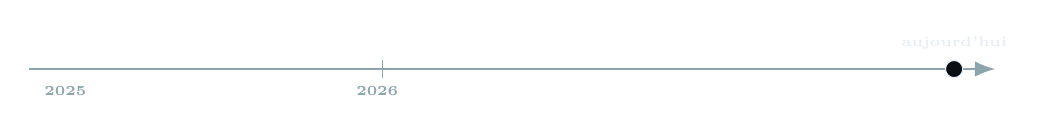
\begin{tikzpicture}[x=0.66cm, y=1.1cm,
         tlev/.style={align=center, text width=2.8cm, font=\scriptsize, text=cyber-ink, inner sep=1pt, execute at begin node={\hyphenpenalty 10000\exhyphenpenalty 10000}},
         tldot/.style={circle, fill=cyber-accent, inner sep=2.2pt},
       ]
       \draw[cyber-soft, line width=1pt, -{Latex}] (-0.8,0) -- (17.8,0);
       \foreach \m/\y in {0/2025, 6/2026}
         \node[font=\tiny\bfseries, text=cyber-soft] at (\m-0.1,-0.25) {\y};
       \draw[cyber-soft] (6,-0.1) -- (6,0.1);

       \tlup{0}{Mai 2025}{Lancement du projet}
       \tldown{3.5}{Juil. -- sept. 2025}{Socle de la plateforme : interface, API et automatisation}
       \tlup{7.5}{Mars 2026}{Installation guidée}
       \tldown{10.5}{Avr. -- juin 2026}{Site web public et documentation}
       \tlup{13.5}{Août -- sept. 2026}{Réseaux et pare-feu configurables}
       \tldown{15.5}{Oct 2026}{Outillage des exercices}

       \node[circle, draw=cyber-ink, fill=cyber-bg, inner sep=2.2pt] at (17,0) {};
       \node[font=\tiny\bfseries, text=cyber-ink] at (17,0.3) {aujourd’hui};
     \end{tikzpicture}
     \note[item]{Message clé : 18 mois se sont écoulés entre le premier commit et la mise à disposition d’un cyber range opérationnel.}
     \note[item]{Mai 2025 : création de l’organisation GitHub (23 mai) et des premiers dépôts : catalogue, playbooks et rôle de contrôleur Proxmox.}
     \note[item]{Juillet – septembre 2025 : Deployer UI (29 juillet), premières stacks Docker pour le CTF (4 août), API backend (3 septembre) et API gateway (22 septembre).}
     \note[item]{Mars 2026 : assistant d’installation et CLI \texttt{range42-context} (30 mars).}
     \note[item]{Avril – juin 2026 : site web (17 avril) et site de documentation (28 juin).}
     \note[item]{Août – septembre 2026 : réseaux SDN Proxmox (18 août) et pare-feu intégrés à chaque déploiement (4 septembre).}
     \note[item]{Octobre 2026 : outillage des exercices, avec l’outil de reporting (débuté le 9 juin) et table42 (10 octobre).}
\end{frame}

% === TODAY VS TOMORROW ===
\begin{frame}{Aujourd’hui et demain}
     \begin{columns}[T]
       \column{0.48\textwidth}
       {\large\textbf{\faCheckCircle\; Aujourd’hui}}
       \begin{itemize}
         \item Installation guidée et exploitation
         \item Concepteur visuel de labs
         \item Réseaux et pare-feu configurables
         \item Labs prêts à déployer
         \item Outils de tabletop exercise (TTX) et de reporting
       \end{itemize}
       \column{0.48\textwidth}
       {\large\textbf{\faRocket\; Demain}}
       \begin{itemize}
         \item Postes de travail pour les apprenants
         \item Exercices Red Team / Blue Team avec système de score
         \item Labs de forensics et de réponse à incident (IR)
         \item Scénarios ICS et IoT
         \item Partage du catalogue
       \end{itemize}
     \end{columns}
     \note[item]{Message clé : le socle est opérationnel ; les prochaines étapes permettront d’enrichir le contenu des exercices et de passer à l’échelle.}
     \note[item]{Aujourd’hui : toutes les fonctionnalités présentées dans cet exposé sont disponibles. Installation et exploitation, conception visuelle des labs (enregistrés sous forme de code), configuration des réseaux et du pare-feu, déploiement de labs d’infrastructure, applicatifs, de détection et de CTF, organisation de TTX et utilisation de l’outil de reporting.}
     \note[item]{Demain : postes de travail pour les apprenants dans le cadre d’exercices pratiques, exercices Red Team / Blue Team avec tableau des scores, labs de forensics et de réponse à incident (IR), scénarios ICS / SCADA et IoT, ainsi qu’un catalogue fédéré permettant de partager des bundles entre organisations.}
\end{frame}

% === ROADMAP ===
\begin{frame}{Feuille de route}
     \begin{tabular}{@{}p{0.53\textwidth}@{\hspace{0.03\textwidth}}p{0.44\textwidth}@{}}
       \runitem{\faIcon{shield-alt}}{Stabilisation et durcissement du cœur}{Figer l’architecture et valider les déploiements} &
       \runitem{\faSync}{Gestion de l’état (DLSE)}{Les labs restent toujours conformes à leur code} \\
       \noalign{\vspace{1.3em}}
       \runitem{\faDesktop}{Interfaces pour les utilisateurs finaux}{Visualiser, modifier et contrôler les labs en cours d’exécution} &
       \runitem{\faUserGraduate}{Services destinés aux apprenants}{Enrichir le catalogue : Git, chat et partage de fichiers} \\
       \noalign{\vspace{1.3em}}
       \runitem{\faIndustry}{Industrie et IoT}{Labs OT / ICS reposant sur du matériel industriel réel} &
       \runitem{\faUsers}{Écosystème open source}{MISP, Kunai et d’autres outils sous forme de labs gérés} \\
     \end{tabular}
     \note[item]{Message clé : six axes de développement orientent les prochaines étapes du projet.}
     \note[item]{Stabilisation et durcissement du cœur : figer l’architecture et le processus d’installation, valider les déploiements à froid et assurer la cohérence entre la CLI, l’UI et l’API.}
     \note[item]{Gestion de l’état (DLSE) : Desired / Live State Engine. Ce moteur compare les labs en cours d’exécution à l’état souhaité, corrige les écarts et conserve une piste d’audit.}
     \note[item]{Interfaces pour les utilisateurs finaux : destinées aux formateurs et aux apprenants, et pas uniquement aux opérateurs. Elles permettront de visualiser l’état déployé, puis de le modifier et de redéployer le lab, avant d’introduire certaines possibilités de contrôle en temps réel.}
     \note[item]{Services destinés aux apprenants : enrichir le catalogue avec les services nécessaires à une classe, comme Git (Gitea), le chat et le partage de fichiers (Nextcloud), à l’échelle d’une classe ou d’un lab.}
     \note[item]{Industrie et IoT : étendre le périmètre de l’IT vers l’OT / ICS avec de véritables composants industriels. Réaliser d’abord un prototype, puis prendre une décision go / no-go.}
     \note[item]{Écosystème open source : intégrer des outils open source existants (MISP, Kunai) sous forme de labs gérés et reproductibles. À plus long terme : synergies avec NGSOTI et catalogues fédérés.}
\end{frame}

% === GET INVOLVED ===
\begin{frame}{Contribuer au projet}
     \vspace*{0.9em}
     \begin{columns}[c]
       \column{0.62\textwidth}
       \runitem{\faBoxOpen}{Contenu}{Scénarios, bundles et challenges CTF}
       \par\vspace{0.9em}
       \runitem{\faCode}{Code}{Automatisation, API et interfaces}
       \par\vspace{0.9em}
       \runitem{\faBook}{Documentation et tests}{Guides, rapports de bugs et retours}
       \par\vspace{0.9em}
       \runitem{\faHandshake}{Partenariats}{Utilisez la plateforme et partagez vos besoins}
       \column{0.36\textwidth}
       \centering
       \colorbox{white}{\qrcode[height=2.6cm]{https://github.com/range42}}
       \par\medskip
       {\small
       \begin{tabular}{@{}c@{\;\;}l@{}}
         \faGithub   & \href{https://github.com/range42}{github.com/range42} \\
         \faGlobe    & \href{https://range42.lu/}{range42.lu} \\
         \faBook     & \href{https://docs.range42.lu/}{docs.range42.lu} \\
         \faEnvelope & \href{mailto:range42@nc3.lu}{range42@nc3.lu} \\
       \end{tabular}}
     \end{columns}
     \note[item]{Message clé : Range42 est open source ; chaque contribution fait progresser la plateforme.}
     \note[item]{Contenu : nouveaux scénarios, bundles pour de nouveaux services et applications, challenges CTF.}
     \note[item]{Code : rôles et automatisation Ansible, API backend, Deployer UI et CLI.}
     \note[item]{Documentation et tests : guides sur docs.range42.lu, rapports de bugs et retours sur GitHub.}
     \note[item]{Partenariats : les organisations peuvent déployer Range42 pour leurs propres formations et nous faire part de leurs besoins.}
     \note[item]{Le QR code renvoie vers github.com/range42. Contact : range42@nc3.lu.}
\end{frame}

% === CLOSING ===
\begin{frame}{}
     \centering
     \includegraphics[trim=9 59 4 43, clip, height=5em]{../../../images/logos/range42.png}
     \par\bigskip
     {\Huge\bfseries Merci}
     \par\medskip
     {\Large Des questions ?}
     \par\vspace{1.5em}
     {\small
     \faGithub\; \href{https://github.com/range42}{github.com/range42}\qquad
     \faGlobe\; \href{https://range42.lu/}{range42.lu}\qquad
     \faEnvelope\; \href{mailto:range42@nc3.lu}{range42@nc3.lu}}
     \note[item]{Remercier le public et ouvrir la session de questions.}
     \note[item]{Questions possibles : état d’avancement de Windows AD, dépôts accessibles publiquement, comparaison avec les cyber ranges commerciaux et modalités pour essayer la plateforme (docs.range42.lu).}
\end{frame}

\end{document}
